\documentclass[12pt,a4paper]{article}

\usepackage[english]{babel}
\usepackage{amsmath}
\usepackage{upgreek}
\usepackage{paralist}
\usepackage{verbatim}
\usepackage{xfrac}
\usepackage{vhistory}

% make in the latest NIPS format (as of this writing, 2017)

\usepackage[nonatbib,final]{nips_2017}
%\usepackage[nonatbib,final]{nips_2017}

\usepackage{color}
\usepackage{graphicx}
\DeclareGraphicsExtensions{.pdf,.eps,.png,.jpg}		% search for .pdf, then .eps, then .pngs, then .jpg

% look in these subdirectories for graphics referenced by \includegraphics
% each entry must end with a /
\graphicspath{{figs/}{figures/}{images/}{./}}

\newcommand*{\red}[1]{ \color{red} #1}

%\usepackage{tabularx}
\usepackage{url}
\usepackage{amsmath}

% this is for environments \subfigure and \subtable
\usepackage{subcaption}

% These packages are FORBIDDEN
%%%%%%%%%%%%%%%%%%%%%%%%%%%%%%%%%%%%%%%%%%%%%%%%%%%%%%%%
%\usepackage{lmodern} % messes up \textsc
%\usepackage{cite} % messes up NIPS
%\usepackage{fullpage} % messes up NIPS
%\usepackage{natbib} % messes up NIPS
%%%%%%%%%%%%%%%%%%%%%%%%%%%%%%%%%%%%%%%%%%%%%%%%%%%%%%%%

\usepackage{array}			% replacement for eqnarray.  Must be BEFORE \usepackage{arydshln}
\usepackage{units}			% for \nicefrac{\alpha}{\beta}


\usepackage{amsthm}		% for theorems
\newtheorem{definition}{Definition}

% text looks a little better
\usepackage{microtype}

\usepackage{wasysym}

\usepackage{textcomp, marvosym} % pretty symbols
\usepackage{booktabs} 	% for much better looking tables

% for indicator functions
\usepackage{dsfont}

% For automatic capitalizaton of section names, etc.
\usepackage{titlesec,titlecaps}


\Addlcwords{is with of the and in}
\Addlcwords{of the}
\Addlcwords{and}
\titleformat{\section}[block]{}{\normalfont\Large\bfseries\thesection.\;}{0pt}{\formatsectiontitle}
\newcommand{\formatsectiontitle}[1]{\normalfont\Large\bfseries\titlecap{#1}}

\titleformat{\subsection}[block]{}{\normalfont\large\bfseries\thesubsection.\;}{0pt}{\formatsubsectiontitle}
\newcommand{\formatsubsectiontitle}[1]{\normalfont\large\bfseries\titlecap{#1}}





% for pretty Euler script
% \usepackage[mathscr]{euscript}
% \usepackage{bold-extra}





%\usepackage{subfig}
\usepackage{float} % for \subfloat

%%%%%%%%%%%%%%%%%%%%%%%%%%%%%%%%%%%%%%%%%%
%% More customizable Lists
%%%%%%%%%%%%%%%%%%%%%%%%%%%%%%%%%%%%%%%%%%
% Better symbols custom enumerative lists, define any symbol you'd like
% \usepackage{enumitem}


%%%%%%%%%%%%%%%%%%%%%%%%%%%%%%%%%%%%%%%%%%
%% Custom Symbols 
%%%%%%%%%%%%%%%%%%%%%%%%%%%%%%%%%%%%%%%%%%
% \xspace at the end of custom macros never screws up spacing.
\usepackage{xspace}



%%%%%%%%%%%%%%%%%%%%%%%%%%%%%%%%%%%%%%%%
%% Abbreviations you'll always want
%%%%%%%%%%%%%%%%%%%%%%%%%%%%%%%%%%%%%%%%
\newcommand*{\TODO}[1]{{\centering {\small \sffamily \color{red} #1} \vskip10pt }}
\newcommand*{\todo}[1]{{\small \sffamily [{\color{red} #1}]}}
\newcommand*{\q}[1]{{\small \sffamily [{\color{blue} #1}]}}
\newcommand*{\fix}[1]{{\sffamily [{\textnormal{\color{red} #1}}]}}



%-----------------------------------------------------------------------------
%  Cross references
%-----------------------------------------------------------------------------
% The following code defines how you make references to figures, tables, etc...
% It is defined in one place only, and can be modified for all references
% in the document at the same time.
% Instead of typing each time: "see Fig. \ref{myfig}" you can create a command
% \figref which will do the job. Then in text you only type \figref{myfig} and LaTeX
% will do the rest.
\newcommand{\tblref}[1]{Table~\ref{#1}}
%\renewcommand*{\figref}[1]{Fig.~\ref{#1}}
\renewcommand{\eqref}[1]{eq.~(\ref{#1})}
\newcommand{\Subref}[1]{(\subref{#1})}


\newcommand{\figref}[1]{Figure~\ref{#1}}
\newcommand{\Figref}[1]{Figure~\ref{#1}}
\newtheorem{theorem}{Theorem}
\newtheorem{lemma}[theorem]{Lemma}

%%%%%%%%%%%%%%%%%%%%%%%%%%%%%%%%%%%%%%%%

% for \sout{} for strikeout
% \usepackage[normalem]{ulem}


% for better manipulation of tables
\usepackage{makecell}
\renewcommand\theadfont{\bfseries}


%-----------------------------------------------------------------------------
%  Misc symbols that I like
%-----------------------------------------------------------------------------
\newcommand*{\opname}[1]{\operatorname{#1}}


\renewcommand*{\to}{\rightarrow}


%%%%
\graphicspath{{images/}}

\title{Mosaic\\\sc\Large{Running Meta-Blockchains to \\ Scale Decentralized Applications}}
\author{\textbf{M. Schenck, P. Gevorgyan, S. Jain,}\\ \textbf{D. Kumar Nath, S. Khedar, B. Bollen}\\ for OpenST Foundation \\ preliminary draft -- version 0}

\begin{document}

\maketitle

\begin{abstract}
Mosaic is a parallelisation schema for decentralized applications.
Mosaic introduces a set of Byzantine fault-tolerant (BFT) consensus rules to compose heterogeneous blockchain systems into one another.
Decentralized applications can use Mosaic to compute over a composed network of multiple blockchain systems in parallel.
In this work we build on existing work to construct an asynchronous, BFT algorithm for an open set of staked validators to finalise a history of transactions executed off of an \emph{origin} blockchain.

Any actor can propose these finalised histories on the origin blockchain to commit them at any point. We detail how invalid proposals can be challenged under different security models, from an honest supermajority of validators up to a single honest observer.

The resulting commits of state transitions form an unforkable chain of \emph{meta-blocks} in a smart contract on the origin blockchain, we call a \emph{meta-blockchain}.
A meta-blockchain prioritises correctness over liveliness and halts if there is a consensus failure.
We detail how state can be recovered on the origin blockchain for a halted meta-blockchain that was running on top of it.

The Mosaic consensus rules are asynchronous and as a result the state transitions of the meta-blockchain can span an arbitrary time length and an arbitrary amount of computation.
The computational effort required by the origin blockchain to (challenge and) commit a meta-block is constant in the computation executed and scales linearly in the number of validators.

Validators are rewarded for the verification effort of the executed computation relative to their contribution to the finalised and committed meta-block.
There is no leader-selection or race condition for rewards in the construction of a meta-block.
As a result of the collaborative reward mechanism the transaction fee market for execution on a meta-block is expected to trend towards the physical hardware cost of redundant computation.

We present an atomic messaging protocol to communicate between the origin blockchain and meta-blockchains running on top of it.
We apply the messaging protocol explicitly to transfer ERC20 tokens from origin to the meta-blockchain.
We detail how ownership of the tokens can be recovered without a time constraint on the origin blockchain if the meta-blockchain would halt due to consensus failure.

You are invited to review critically all content and join discussions on \mbox{\url{discuss.openst.org}}.
The code is open-source and under development at \url{github.com/openstfoundation/mosaic-contracts}.
\end{abstract}

\newpage
%
% Section
%
\section{Introduction}

Mosaic is a parallelisation schema for decentralized applications.
Mosaic introduces a set of Byzantine fault-tolerant (BFT) consensus rules to compose heterogeneous blockchain systems into one another.
Decentralized applications can use Mosaic to compute over a composed network of multiple blockchain systems in parallel.

A decentralized application is an application for which the computation is requested, performed, and paid for by independent actors.
To date, Ethereum is the leading network
% TODO: quantify and reference; also define Ethereum as an instruction set, a mainnet network.
of nodes that enables developers to write and deploy code which can be called by independent users to collectively construct a shared state of the application.

The Ethereum network achieves agreement on the collective state by constructing a blockchain.
A blockchain derives correctness from full replication of the computation by nodes.
Furthermore, to ensure correct execution of blockchain computations, an order on the inputs of execution must be determinable.
% TODO: give short intro, start from satoshi
In its current implementation, the Ethereum chain is appended through Proof-of-Work consensus.
Proof-of-Work (PoW) introduces a block reward incentive for nodes to keep producing blocks and thereby securing the chain of historical blocks.
However, PoW produces a serial execution model and nodes cannot be collectively rewarded for the computation they all have to perform, which renders the system computationally inefficient\cite{verifiersdilemma}.

% NOTE: Ethereumv2 still needs to serialise all execution; DFinity starts from scratch.
Active research and implementation work is ongoing to scale Ethereum's transaction throughput by dividing the verification work into multiple sections, also referred to as \emph{shards}.
At the same time, Ethereum is committed to moving from the probabilistic Proof-of-Work consensus engine to a BFT based Proof-of-Stake (PoS) consensus engine\footnote{
	\url{https://github.com/ethereum/eth2.0-specs/blob/master/specs/beacon-chain.md}
}.
The outset of a BFT consensus engine is to collectively produce a blockchain which provably --- under certain honesty assumptions --- cannot finalize conflicting blocks.

Thus far a vision for a decentralized web has been a major driver of innovation.
However, to power global networks of billions of users and decentralized computation on vast decentralized data stores, it is reasonable to assume no single blockchain network will suffice as a backbone for all types of applications.
Much like the internet is a composed network of networks, we can conceive decentralized applications to transcend any single blockchain and execute across a network of blockchain networks.

We detail two protocols in this work.
The first, a layer-2 protocol, constructs \emph{meta-blockchains} on top of existing blockchain networks to extend their state space and transaction throughput capacity.
The second protocol, called a \emph{gateway}, acts as a message bus to send typed messages atomically between the underlying layer-1 blockchain and the meta-blockchain running on top of it.

Together these two building blocks can be used by decentralized applications to construct a parallelisation schema to increase %on-chain
computational capacity at lower transaction cost.
In its simplest form, a decentralized application can offload transaction processing to a single meta-blockchain.
More advanced applications can deploy logic across many meta-blockchains and process transactions in parallel while they can send asynchronous messages across meta-blockchains.

%%%%%%%%%%%%%%%%%%%%%%%%%%%
% TODO: describe sections %
%%%%%%%%%%%%%%%%%%%%%%%%%%%

%
% Section
%
\section{Composing meta-blockchains}

A meta-blockchain composes transactions executed on an auxiliary blockchain system into an origin blockchain, such that the capacity of the origin blockchain extends and the auxiliary blockchain inherits the security properties of the origin blockchain.

To this end consider two blockchain systems, an origin blockchain $O$ with state transition rules $t_O$ which progress the state $\Sigma_O$ 
\begin{align} \label{state_transition_rules}
  t_O : \Sigma_O \rightarrow \Sigma_O'
\end{align}
and similarly consider an auxiliary system $A$ with state transition rules $t_A$ such that $t_A : \Sigma_A \rightarrow \Sigma_A'$.


Transition rules for the origin and auxiliary system can be similar but do not have to be.
In our discussion, when we need an example, we will refer to the origin blockchain as Ethereum (Byzantium), running Proof-of-Work, and for the auxiliary system we consider Go-Ethereum, running ``clique'' Proof-of-Authority (PoA).
We deliberately use PoA for our considerations for the auxiliary system to emphasize that the security for the composed auxiliary system is not derived from the consensus engine of the auxiliary system.
Rather the security properties of the composed system must rely only on the security properties of the consensus rules of the origin blockchain and on the Mosaic BFT consensus rules composing the auxiliary system into the origin system.\footnote{
	The block proposers of the auxiliary system do have the ability to censor transactions from the auxiliary system if they have an ability to collude.
}

We define a meta-blockchain $\mathcal{B}$ with a staked validator set $\mathcal{V}_\mathcal{B}$ on the origin blockchain. The blocks $B_i$ of $\mathcal{B}$ are committed to a \emph{core} contract on origin $O$.
For a given history of $O$,\footnote{
	The origin blockchain $O$ might be probabilistically finalized, in which case a transaction to a contract can always assert that it is valid only on the intended branch of history by referencing a historical blockhash.
}
the meta-blockchain cannot fork if we enforce that block $B_{n+1}$ can only be (proposed and) committed after block $B_n$ has been committed.

We define a meta-block $B_i(K, T, S): \Sigma_A \rightarrow \Sigma_A'$ to progress the state of the auxiliary system $A$, where we call $K$ the \emph{kernel}, $T$ the \emph{transition object} and $S$ the \emph{seal}.
A block $B_i$ at height $i$ of the meta-blockchain is committed with a seal $S$ when a $\texttt{+}\sfrac{2}{3}$ supermajority of the weighted votes has been verified.\footnote{
	While a vote counted on a BFT system itself is already BFT for a simple majority, % TODO : reference
	we still require a supermajority, because the votes to commit a meta-block will be collected on the auxiliary system for which there is no assumption it is BFT, and we want Mosaic to be able to finalize transactions on the auxiliary system before they are committed to origin.
}
We will detail later how the meta-block is constructed, but first we will describe the vote messages which, combined, seal a meta-block.

\subsection{Checkpoint finalisation - Casper FFG}
The reader is assumed at this point to be familiar with the work presented in \textit{Casper the Friendly Finality Gadget}\cite{casperffg} (FFG), as we will build on the logic and proofs presented there.
We will intend to align with definitions and notations where possible and highlight deviations where appropriate.
This section briefly (and incompletely) summarizes core concepts from the paper, so that the shared concepts are established for the reader.

Casper FFG presents an algorithm to build up an overlay network of vote messages presented to a smart contract about the blocks already produced by the underlying network of nodes running the blockchain.
The overlay network aims to repeatedly economically finalize a single branch of the underlying network.
It does so by allowing staked validators to cast votes which together can construct a \emph{justified chain}.

A justified chain is formed by a sequence of \emph{supermajority links}, where a link identifies a \emph{source} blockhash $s$ and its height $h_s$ and a \emph{target} blockhash $t$ and its height $h_t$.
A vote message in Casper FFG is a link $\langle s, t, h_s, h_t\rangle_v$ signed by a validator $v$.
A $\texttt{+}\sfrac{2}{3}$ supermajority signing of the same link makes it a supermajority link which justifies the target block if the source block is itself already justified.\footnote{
	The genesis block of the auxiliary blockchain is considered justified by definition.
}

In the work it is shown that checkpoints along a justified chain can additionally be considered \emph{finalized}, if and only if they are justified themselves and their direct child checkpoint is justified.
It is then shown that, should validators finalize a checkpoint on a contradicting branch of the history of the underlying blockchain, minimally $\sfrac{1}{3}$ of the validator weight must have signed vote messages that violate either one of two rules: \emph{the Casper slashing conditions}.

These slashing conditions can be intrinsically validated given two signed vote messages from a validator $v$.
As such a validator must never sign two vote messages $\langle s_1, t_1, h_{s_1}, h_{t_1}\rangle_v$ and $\langle s_2, t_2, h_{s_2}, h_{t_2}\rangle_v$ for which either $h_{t_1} = h_{t_2}$ or $h_{s_1} < h_{s_2} < h_{t_2} < h_{t_1}$ holds.

It is additionally shown that validators can always finalize a new checkpoint, without being required to violate the slashing conditions, given that the block proposers propose blocks to append to the finalized fork, i.e. follow the fork selection rule of the overlay network.

\subsection{Finalizing auxiliary systems}
Given a validator set $\mathcal{V}_\mathcal{B}$ staked for the meta-blockchain on origin, validators $v \in \mathcal{V}_\mathcal{B}$ can submit, on the auxiliary system, vote messages about the auxiliary system of the form
\begin{align}\label{externalizedvote}
  \langle \tilde{T}, s, t, h_s, h_t \rangle_v
\end{align}
where $\tilde{T}$ is the keccak256 hash of the transition object $T$.

We introduce a transition object hash in the vote message to externalize otherwise intrinsic properties of the auxiliary system.
This transition object allows the Mosaic validators to coarse-grain and abstract the auxiliary system into a meta-blockchain when proposing meta-blocks on origin.

We require that any transition object is calculable by a smart contract on the blockchain in question for any finalized checkpoint along a justified chain.
For a given link, we define the transition object to refer to the state of the blockchain at source block $s$.
It then follows that for a given source blockhash $s$, $\tilde{T}$ is uniquely determined by $s$ and the same properties of accountable safety and plausible liveliness hold for a finalized checkpoint on a justified chain constructed by such \emph{externalized vote messages} (\ref{externalizedvote}), if we extend the slashing conditions to accommodate for the transition object hash.

A validator $v \in \mathcal{V}_\mathcal{B}$ must never sign two externalized vote messages $\langle \tilde{T}_1, s_1, t_1, h_{s_1}, h_{t_1}\rangle_v$ and $\langle \tilde{T}_2, s_2, t_2, h_{s_2}, h_{t_2}\rangle_v$ such that any of the following three conditions holds:
\begin{enumerate}
  \item $h_{t_1} = h_{t_2}$,
  \item $h_{s_1} < h_{s_2} < h_{t_2} < h_{t_1}$,
  \item $s_1 = s_2 \land T_1 \neq T_2$.
\end{enumerate}

As the slashing conditions can be intrinsically asserted to have been violated given two externalized vote messages by the same validator, there is no communication overhead to assert a possible violation of these conditions on the origin blockchain; even if the justified chain is being constructed on the auxiliary system.
As a result, the validators in $\mathcal{V}_\mathcal{B}$ can be held accountable on the origin blockchain for their voting actions on the auxiliary system.
The slashing condition can be asserted on both systems and there is a clear incentive for the honest validators to assert any violation without delay on both the origin and auxiliary system, naturally synchronising the validator weights when such an event occurs.

We will later in this work address a dynamic validator set $\mathcal{V}_\mathcal{B}$, where validators can join and log out on the origin system.
However, already with a static validator set, we can observe that the finality gadget first introduced for (re)defining economic finality in layer-2 of Ethereum's PoW -- turning miners into mere block proposers and introducing a PoS (partial) consensus engine in the smart contract layer -- can also be applied to finalize an independent (auxiliary) system with a validator set whose stake is held on an external (origin) blockchain.

% TODO: EXPAND into a full section later
%\subsection{Expansion somewhere}

\subsection{Observing origin}
\label{observing_origin}

Per construction, the finalization of the auxiliary system by the Mosaic validators economically binds the block proposers of the auxiliary system to the Mosaic fork selection.
By finalizing the auxiliary system the Mosaic validators reach consensus about the auxiliary system itself.
However, to be able to pass messages bidirectionally between chains, the Mosaic validators are additionally required to reach consensus about their observation of the origin blockchain on the auxiliary system.

To achieve this, the Mosaic validators construct a justified chain and finalize checkpoints along it for reported blocks of the origin blockchain on the auxiliary system.
The incentive structure is now reversed and the origin blockchain is in no way incentivized (nor should it be) to follow the fork selection rule of how a meta-blockchain's validator set finalized its observation of the origin blockchain.

In case the origin blockchain is probabilistically finalized, then it is always possible that the Mosaic validators of a given meta-blockchain running on top of the origin blockchain would economically finalize an observation of origin on the auxiliary system which is (later) reverted by the origin blockchain - even if they sufficiently trailed the head of origin.
Note that the validators cannot revert their finalized observation, because they would be required to sign vote messages which would violate the slashing conditions.

Under this scenario we must force the meta-blockchain to halt at the highest finalized checkpoint of the auxiliary system which was still consistent with its observation of the (now reverted) history of the origin blockchain.
This property can be enforced by including in the transition object of a justified chain of the auxiliary system $T^A$ information about the finalization of the observation of the origin blockchain $T^O$,
\begin{align*}
  T^A_i = (O^j_f, \dots),
\end{align*}
where $O^j_f = f(T^O)$ is the function that returns the highest finalized block number $j$ and blockhash of the origin system as observed by the Mosaic validators for this meta-blockchain.

The origin blockchain can inspect $T^A$ to assert that the highest finalized observation of itself on the auxiliary system is within its current history.
Should this not be the case, then the origin blockchain must reject meta-blocks containing contradictory observations.

However, origin cannot directly assert that prior to the last finalized observation, there was no checkpoint finalized from a contradictory branch of its history, as the nodes on origin should not fully verify the transactions executed on the auxiliary system.
This is resolved by introducing an option to challenge a proposed finalized observation.

Assume an observed checkpoint $a$ was finalized on a contradictory branch of origin relative to the last finalized observed checkpoint $b$ included in $T^A$.
Any honest node can challenge the finalization of $b$ on origin by presenting the finalization of $a$ and demonstrating that $a \notin \text{history}(b)$.
Note that if validators would want to alter the finalized observation from $o \rightarrow a \rightarrow b$ to $o \rightarrow b$ they would have to produce vote messages violating the slashing conditions given the already existing vote messages.

Upon success, the challenger is rewarded from the stake of the offending validators and the core contract must declare the meta-blockchain halted.

\subsection{Calculating the transition objects}

We construct a transition object $T^A$ to coarse-grain a vast amount of transactions processed on the auxiliary system under the state transition rules $t_A$ into a single, abstracted state transition that can be validated by the core contract on the origin blockchain (under the state transition rules of the origin blockchain $t_O$, eq. \ref{state_transition_rules}).

On the auxiliary chain with every block running parameters are tracked and these consist of the latest finalized observation of the origin blockchain $O^j_f= f(T^O)$, the \emph{accumulated transaction root} $r_i$, the \emph{accumulated gas} $g_i$ consumed, and the current \emph{dynasty number} $d$ on auxiliary.
The transition object $T^A$, however, is updated at every justified checkpoint $s$ with height $h_s$ and we write for a given meta-block height $n$:
\begin{align*}
  T^A_{n,d}(s) = (d, O^{j_d}_f, r_d, g_d, \tilde{K}_n)
\end{align*}
where $\tilde{K}_n$ is the keccak256 hash of the kernel $K_n$.

A smart contract calculates the parameters that go into $T^A$ for every block.
Therefore, the validators have to report the block header of every block to the smart contract.
If the reported block is within the most recent 256 blocks of the auxiliary blockchain,\footnote{
	This is specific to the Ethereum virtual machine, but the logic can be applied for other blockchain systems as well.
}
then the smart contract can verify its correctness by accessing the corresponding block hash.
If the validators fall behind more than 256 blocks in reporting, they can report more than one block per new block in order to catch up.
The smart contract will record all reports, but only mark them as valid if they build a chain that reconnects to a block hash within the most recent 256 blocks of the current branch.

Tracking of $T^A$ begins at the genesis checkpoint.
For the genesis checkpoint, the accumulated transaction root is defined as the transaction root of the block, the accumulated gas consumed equals the gas consumed in the block, and the current dynasty number is 0.
For all subsequent blocks, the accumulated transaction root $r_i$ at block height $i$ is $\text{keccak256}(r_{i-1}, R_i)$, where $R_i$ is the transaction root of the block at height $i$.
The accumulated gas consumed $g_i$ at block height $i$ is $g_{i-1} + G_i$, where $G_i$ is the gas consumed in the block at height $i$.
The dynasty number equals the number of finalized checkpoints in the chain from the root checkpoint to the parent block, carrying over the definition of dynasty number as in Casper FFG \cite{casperffg}.

Further, we introduce a constant \emph{core identifier}, a 256-bit string where the first 12 bytes are a constant specifying the origin blockchain and the rightmost 20 bytes are determined by the smart contract address of the core contract on the origin blockchain.
Rather than storing the core identifier in the transaction object, it can be included as a constant in the signing string for vote messages to ensure vote messages are valid only about the intended meta-blockchain.
An origin blockchain also has a core identifier to identify vote messages about origin.
For core identifiers that identify an origin blockchain, the rightmost 20 bytes are all zero.

The constant that specifies Ethereum main net as the origin blockchain is \texttt{bytes12(1)}.

% TODO: follow up on the thinking that by externalising the transition object into the vote message allows the calculation to be done in the node, not in the contract.

\begin{figure}
    \centering
	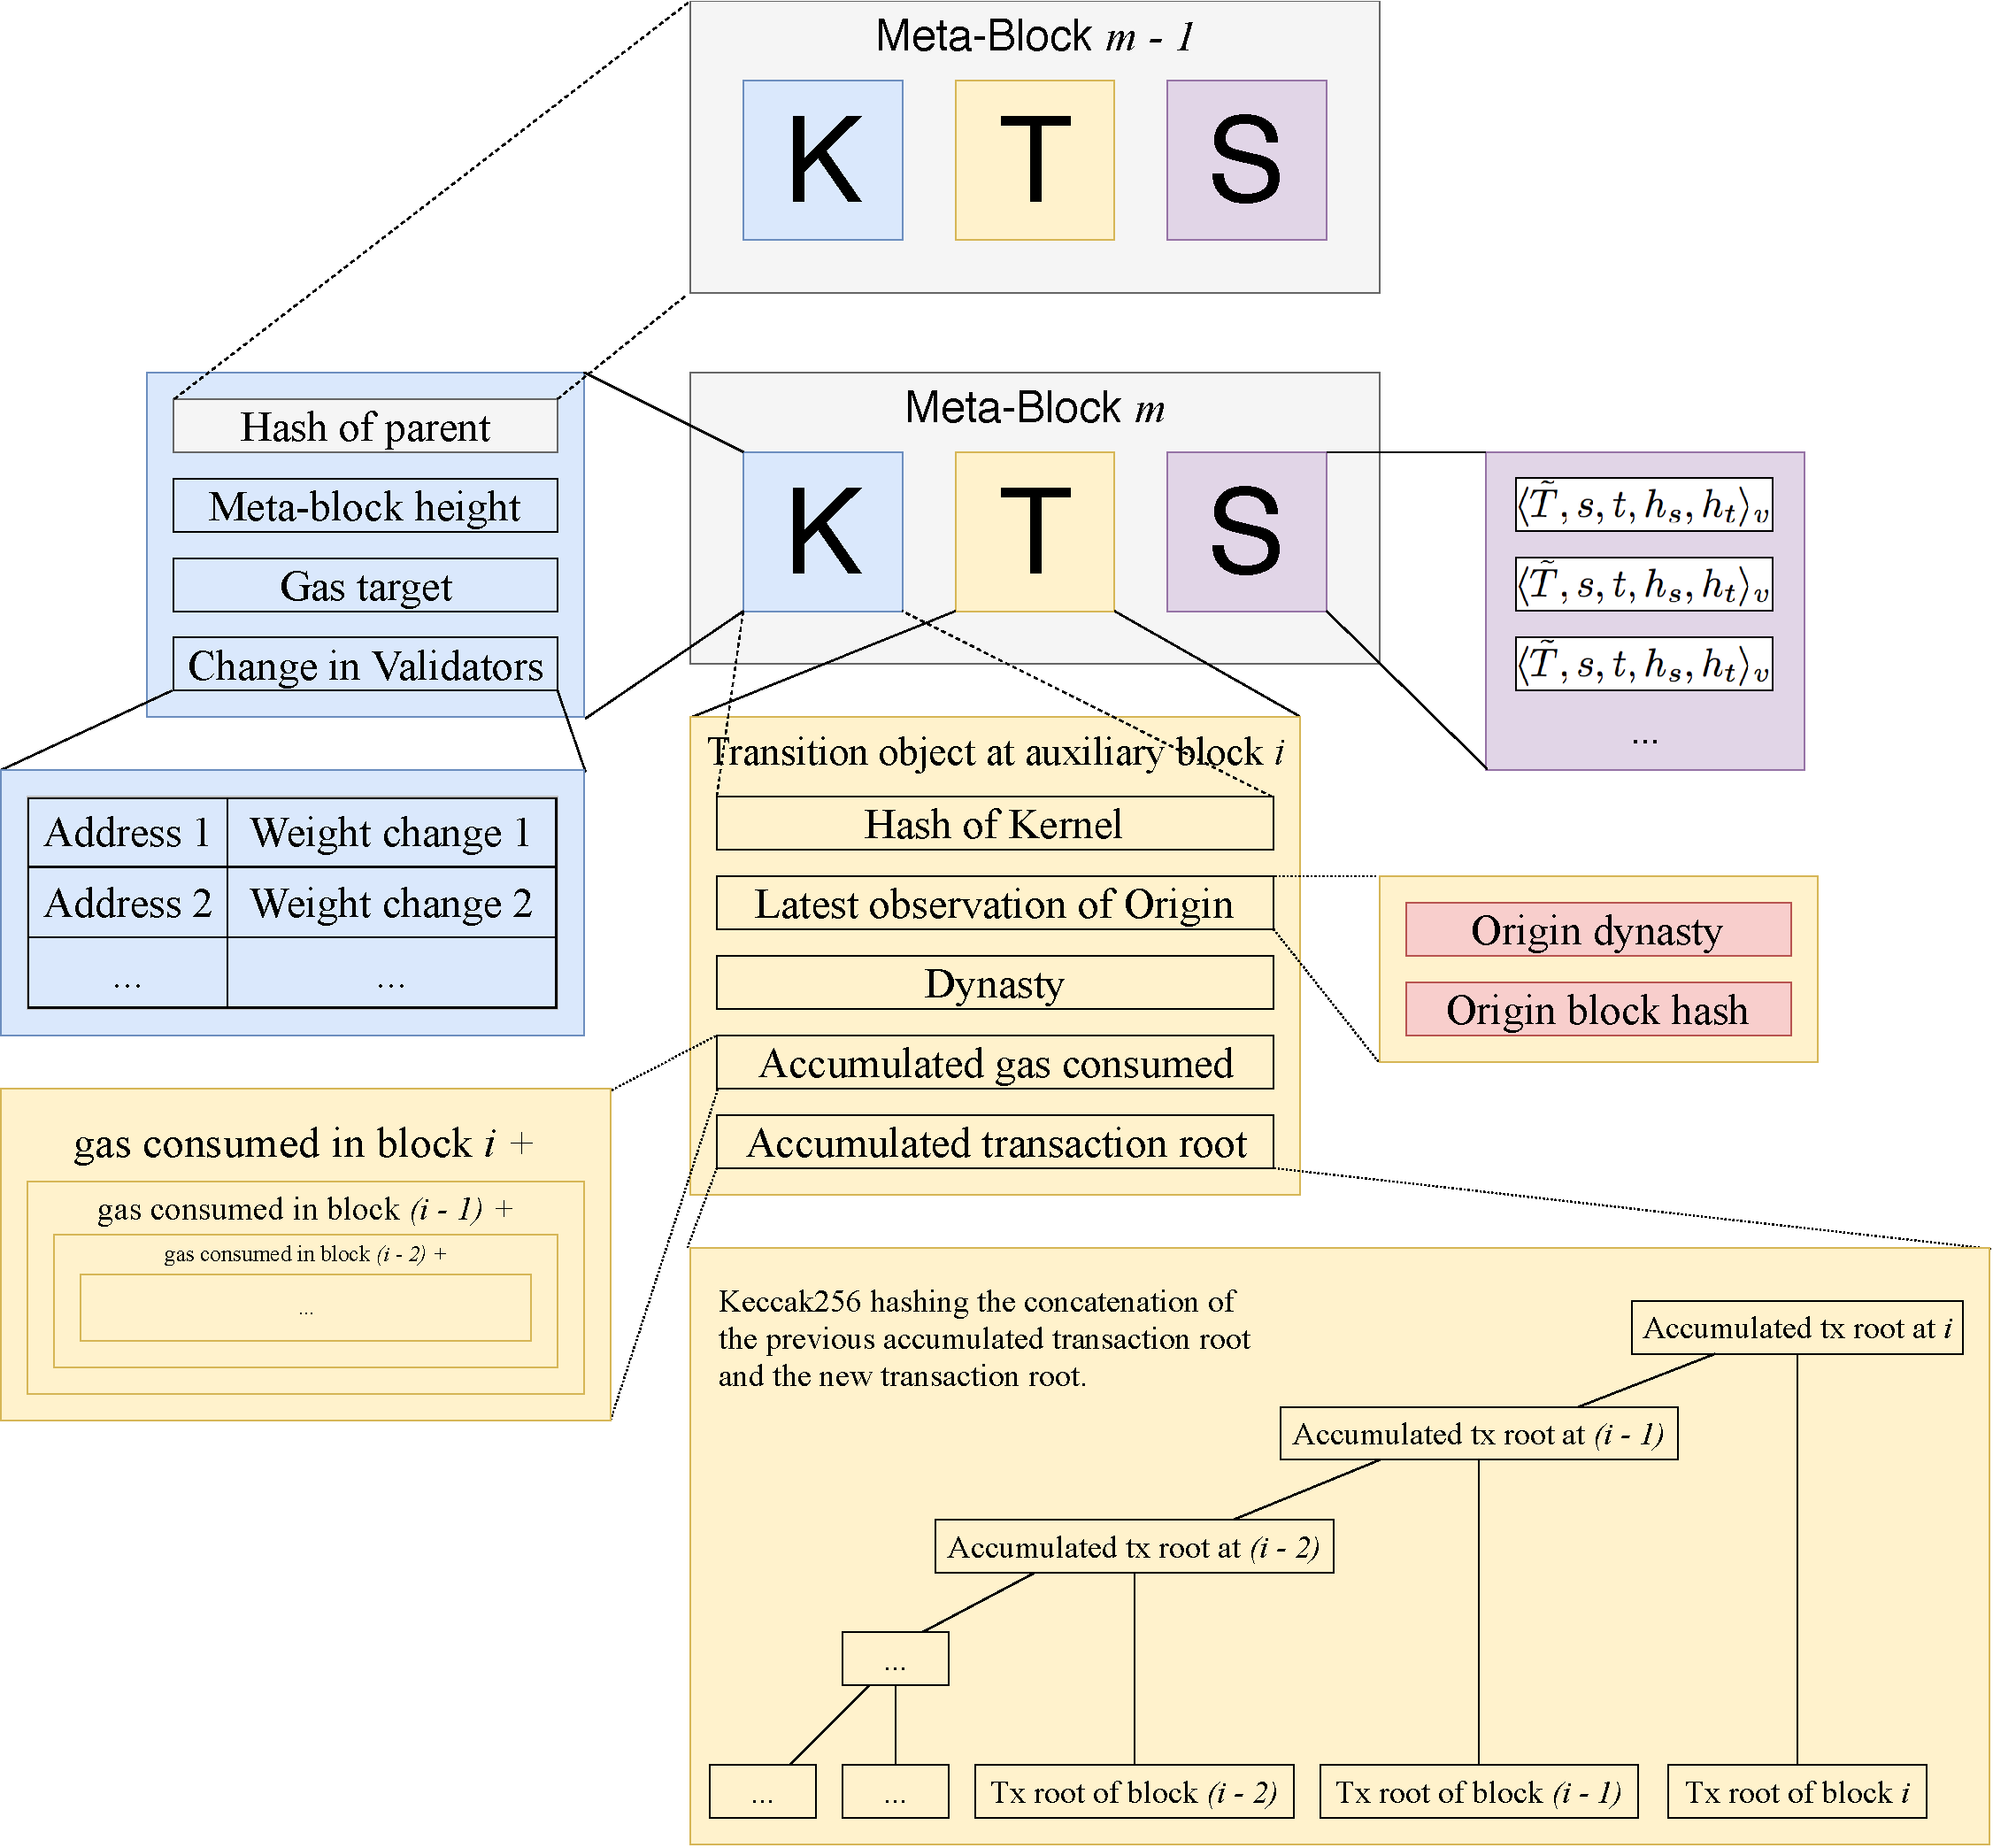
\includegraphics[width=\textwidth]{meta_block}
	\caption{\textbf{Anatomy of a meta-block.}
		The meta-block consists of a kernel, a transition object, and a seal.
	}
	\label{fig:meta_block}
\end{figure}

\subsection{Proposing meta-blocks on origin}
\label{proposing_metablocks}

For a meta-blockchain $\mathcal{B}$ the chain can be appended by proposing and committing new meta-blocks $B_n(K_n, T^A_n, S_n)$ in the core contract on the origin block\-chain.
The genesis meta-block $B_0$ is considered committed per definition.

The kernel $K_n$ is a tuple $(n, \tilde{p}_n, \Delta\mathcal{V}_{\mathcal{B}_n}, gt_n)$ fully determined by and stored in the core contract on the origin blockchain.
On a given branch of the origin blockchain a meta-blockchain cannot fork.
The act of committing a meta-block $B_{n-1}(K_{n-1}, T^A_{n-1}, S_{n-1})$ activates the new kernel $K_n$ at height $n$ and \emph{opens} the core contract to accept proposals of the form $B_n(K_n, \cdot, \cdot)$.
The kernel further specifies the \emph{parent hash} $\tilde{p}_n$ and the \emph{updated validator weights} $\Delta\mathcal{V}_{\mathcal{B}_n}$ to declare new validators joining and existing validators logging out.

\paragraph{gas target} Lastly $gt_n$ is the \emph{gas target} which introduces a forcing function on the total amount of gas that can be consumed in the meta-block $B_n$.
The earliest finalized checkpoint at which the gas target has been consumed by the meta-block must be committed to the origin blockchain by the validators.
We highlight that this is not a maximum gas limit, because it cannot be guaranteed that a checkpoint can be finalized before a hard gas limit would be surpassed. Rather validators would gradually lose part of their stake as a function of the number of finalized checkpoints they failed to commit after the gas target has been surpassed.

To show that validators can be held accountable, assume the finalized checkpoint $s_d$ has been committed which surpassed the gas target and has dynasty number $d$.
Now assume there exists a finalized checkpoint $s_{d'}$ which also has surpassed the gas target but has a lower dynasty number $d' < d$, but was not committed before $s_d$.
Any honest node can present the $s_{d'}$ including the seal and the core contract can assert the gas target had been consumed at a lower dynasty number than what is committed and reward the challenger.\footnote{
    It could happen that the gas target is met and finalized on auxiliary before the new kernel is confirmed.
    However, the first valid finalized checkpoint to be committed on origin is still the first finalized checkpoint after the kernel is confirmed.
    All finalizations before the confirmation of kernel $K_i$ are not valid proposals, as the seal includes the transition object $T^A_{i-1}$.
}

\paragraph{committing a meta-block} Given a committed meta-block $B_{n-1}$ at height $n-1$ a proposal for a meta-block $B_{n}(K_{n}, T^A_{n}, \cdot)$ at height $n$ is a valid proposal if validity assertions for the transition object $T^A_n$ hold.  These validity assertions require that the dynasty number and the gas consumed are strictly increasing compared to the transition object committed $T^A_{n-1}$. The transition object $T^A_n$ must reference the correct kernel $\tilde{K}_n$. It must be checked that the latest finalized observation of origin is within the history of the current state. Furthermore a brief challenge period exists where the transition object can be contested on the grounds that it contains a prior observation of origin that contradicts the current history of origin, as explained above in section (\ref{observing_origin}).

It now follows that for a given active kernel $K_n$ multiple proposals $T^{A}_{n,d}$ can be submitted to the core contract for different dynasty numbers $d$. These proposals are no longer contradicting versions of the history, rather they are ordered, sequenced snapshots of possible state transitions $B_{n,d_{n}}(\Sigma_{A,d_{n-1}})$ that can be committed onto origin as a new meta-block.

To commit a meta-block then requires selecting among the valid proposals a dynasty number $d_n$ for which the meta-block will be closed. This selection occurs automatically by sequentially verifying the vote messages on the origin blockchain.
The meta-block $B_n(K_n, T^A_n, S_n)$ will be committed with the seal $S_n$ which first asserts a $\texttt{+}\sfrac{2}{3}$ supermajority of the voting weight $\mathcal{V}_{\mathcal{B}_n}$ for a valid proposal in the set of valid proposals
\begin{align*}
  \{S_{n,d}\} = \left\{\left\{\langle\tilde{T}^A_{n,d}, s, t, h_s, h_t\rangle_v\right\}\right\}
\end{align*}
where it is required that the supermajority link finalizes the source $s$.
As such we require that $h_t - h_s = 1$ and the source $s$ must have been justified.

Following the same reasoning as presented in section (\ref{observing_origin}) we can assert whether or not the finalized checkpoint $s$ was obtained through an unbroken justified chain leading up to the finalized checkpoint, by allowing for a challenge\footnote{A challenger must always put forward a sufficient stake to underwrite the cost implied by her challenge.} to be raised against a proposed transition object $T^A$ included in a vote message $\langle\tilde{T}^A, s, t, h_s, h_t\rangle_v$.

However, recall that in the case of verifying observations of origin (\ref{observing_origin}), origin itself can act as an arbiter because origin can rely on its own history.
Our concern now is to assert that the state transition to $s$ from the last committed state $B_{n-1}$ is a valid state transition according to the state transition rules $t_A$ of the auxiliary system.

\paragraph{proof} Assume first a contradictory finalisation $s'$ of the auxiliary system relative to $s$ exists. This implies that more than $\sfrac{1}{3}$ of the validator weight can be slashed.
The core contract on origin must declare the meta-blockchain halted when it can slash more than the safety threshold of $\mathcal{V}_{\mathcal{B}_i}$ at a single meta-blockchain height $i$.\footnote{When a meta-blockchain has been halted, assets and stateful objects can be recovered on the origin blockchain at any later time with Merkle proofs against the last committed state root of the meta-blockchain.
We will detail the conditions under which a meta-blockchain must halt and how the recovery processes can work later in this writing.}

Alternatively, no contradictory finalisation $s'$ of the auxiliary system relative to $s$ exists.
Under the security model assuming a $\texttt{+}\sfrac{2}{3}$ supermajority of the validator weight is honest, it follows that the proposed state transition to $s$ has been obtained through honest verification of all transactions under the state transition rules $t_A$.

Before continuing we summarize that the proposal mechanism to commit a meta-block is asynchronous, requires no leadership-selection and is proven to be Byzantine fault-tolerant under the security model of an honest supermajority.

\subsection{Dynamic set of validators}

The set of validators for the meta-blockchain $\mathcal{B}$ must be dynamic to allow new validators to join and for validators to safely exit from their responsibilities.
It is defined for each meta-block height $n$ and we note $\mathcal{V}_{\mathcal{B}_n}$.

A validator $v$ is defined as an address which has a strictly-positive validator weight $w_v$ associated with it on the origin blockchain.
A validator can join the set of validators by sending a \emph{deposit message} to the origin blockchain and putting forward a stake.
A validator can initiate log out by sending a \emph{logout message} to origin.

The weight of a validator $w_v$ at meta-block height $n$ is the product of the stake of the validator at that height $s_v(n)$ multiplied with a \emph{reputation function} $R(n; v, n_0)$
\begin{align}
\label{validator_weights}
  w_v(n) = s_v(n) \cdot R(n; v, n_0)
\end{align}
where the reputation function $R$ has values in the range $[0,1]$ and $n_0$ is the meta-block height where the validator $v$ sent the deposit message.

The reputation function allows for different security models to mitigate collusion attempts of malicious actors within the validator set of the meta-blockchain.
As examples, the reputation function can require initial work by the validator before obtaining a non-zero reputation.
The reputation function can also enforce a finite (probabilistic) lifetime for all validators, honest and dishonest alike.
Inducing churn in the (honest) validator set adds an important stochastic tool to prevent collusion of more than $\sfrac{1}{3}$ of the validator weight.

Changes to the validator weights $w_v(n)$ are included in the kernel $K_n$ as $\Delta\mathcal{V}_{\mathcal{B}_n}$.  When tallying votes both the origin blockchain and the auxiliary system must use the \emph{effective weight} $W_v(n)$,
\begin{align*}
  W_v(n) = w_v(n) \cdot \theta_v
\end{align*}
where $\theta_v$ is initially 1 for all validators, but irreversibly and immediately set to 0 when a validator $v$ is shown to have violated any slashing condition.
The effective weight allows for the voting power of an offending validator to be revoked on both blockchains instantaneously without waiting for the meta-block to be committed.

The stake $s_v(n)$ of a validator can only be preserved or decrease for increasing $n$ when the validator does not fulfill its responsibilities.
The \emph{loss function} $L$ recalculates the stake of a validator for the new meta-block height
\begin{align}
  s_v(n) = L(s_v(n-1); v).
\end{align}
The loss function reduces the actual value the validator can possibly withdraw in the future.  The loss function can reward challengers for presenting proofs of bad behaviour by the validator from his stake and it can burn the remaining reduction.

When a validator violates any slashing condition the loss function returns the validator stake to zero.

Validators can see their stake reduced when they become inactive in the voting process (\emph{inactivity leak}\footnote{
  The inactivity leak forces validators to participate in the voting process and be available.
  The stake of inactive validators can gradually be diluted if they fail to verify their vote on a committed meta-block.
  We credit the term to Casper FFG\cite{casperffg} for the original argument.
}), or when they fail to commit a meta-block back to origin according to the gas target requirements (section  \ref{proposing_metablocks}).

When a validator successfully logs out the reputation is set to zero, but the stake remains locked in the contract for a fixed amount of time to protect against long range revision attacks.\footnote{
  By holding on to the stake the validator can still be held accountable for evidence of wrongdoing that may surface later or new attempts of revising the history.
  We follow Casper FFG's proposal of approximating four months delay before withdrawal is allowed.}
After this time the validator can withdraw his stake (and remaining rewards).

\paragraph{asynchronous composition of blockchains} We refresh for the reader (section \ref{proposing_metablocks}) that a meta-block $B_i$ is committed on origin with a valid\footnote{
  A valid proposal is a transition object $T^A$ which satisfies the validity checks and has been unchallenged, or has been successfully proven upon being challenged.
} transition object $T^A_i(\tilde{K}_i, \cdots)$ for which a seal $S_i$ was created on origin by verifying a supermajority of the voting weight $\mathcal{V}_{\mathcal{B}_i}$ on vote messages of the form $\langle \tilde{T}^A_i, s, t, h_s, h_t \rangle_v$.
As the hash of the kernel $\tilde{K}_i$ is included in the transition object, and as the hash of the transition object $\tilde{T}^A_i$ is included in the vote messages, the order to construct a meta-block $B_i(K_i, T^A_i, S_i)$ is logically enforced.

When a proposed transition object $T^A_i$ is committed as meta-block $B_i(K_i, T^A_i, S_i)$ then the state root of the auxiliary system is immutably anchored into the origin blockchain under the blockhash $s$\footnote{
  We assume here without loss of generality that the blockheader of the auxiliary system includes the state root of the system at height $h_s$ and that the blockhash is the hash of an encoding of the blockheader.}.
It follows that the state of the meta-blockchain is first knowable on the auxiliary system and causally passed to the origin blockchain upon committing $B_i$ (see solid lines on fig. \ref{fig:asynccomp}).

A new kernel $K_{i+1}$ is defined by the committed meta-block $B_i$, the deposit, logout and slashing messages\footnote{
  Slashing messages can concern both violations of slashing conditions reducing the stake of a validator to zero, or a proof of inactivity gradually reducing the validator stake.}
that were included on origin during height $i$\footnote{
  We say a transaction on origin is included during height $i$ if it is included in the history of origin before $B_{i}$ is committed and after $B_{i-1}$ was committed.}
and a new gas target $gt_{i+1}$ for closing $B_{i+1}$.
These messages combined with the recalculation of the validator weights (eq. \ref{validator_weights}) update the validator set
\begin{align}
  \mathcal{V}_{\mathcal{B}_{i+1}} = \Delta\mathcal{V}_{\mathcal{B}_{i+1}}(\mathcal{V}_{\mathcal{B}_{i}})
\end{align}
which is included in $K_{i+1}$ as the operator $\Delta\mathcal{V}_{\mathcal{B}_{i+1}}$. 

\begin{figure}[tb]
    \centering
	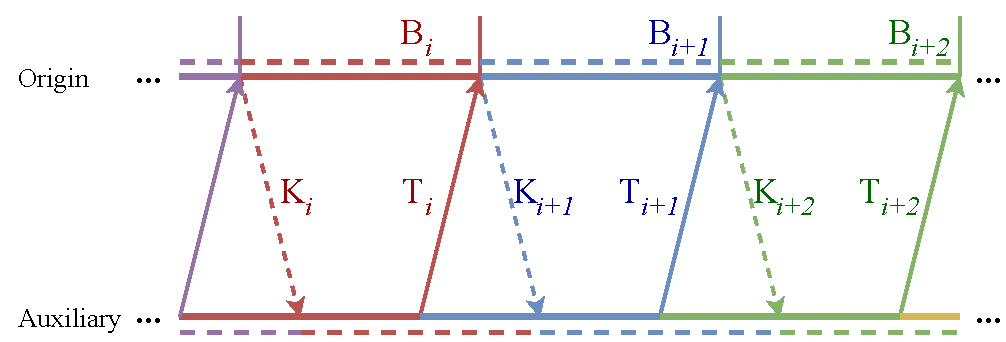
\includegraphics[width=0.8\textwidth]{transition}
	\caption{\textbf{Asynchronous composition.}
		When a proposed transition object $T_i$ is committed as meta-block $B_i$ on origin (solid red line), the new kernel $K_{i+1}$ is opened on origin.
		The validator set $\mathcal{V}_{\mathcal{B}_i}$ (dashed red line on aux) casts votes on the auxiliary system to finalise both the checkpoints of the auxiliary system and its observation of the origin blockchain on the auxiliary system.
		The commit of $B_i$ and opening of $K_{i+1}$ is observed by $\mathcal{V}_{\mathcal{B}_i}$ and $K_{i+1}$ is confirmed on the auxiliary system transitioning to the new validator set $\mathcal{V}_{\mathcal{B}_{i+1}}$ (dashed blue line on aux).
		On the auxiliary system all processes continue uninterrupted.
		At each confirmation of a new kernel $K_j$ the changes to the validator set $\Delta\mathcal{V}_{\mathcal{B}_j}$, and the new gas target $gt_j$ are enacted on the auxiliary system.
	}
	\label{fig:asynccomp}
\end{figure}

The validator set $\mathcal{V}_{\mathcal{B}_i}$ is activated on the auxiliary system when the kernel $K_i$ is \emph{confirmed} on the auxiliary system.
We define the confirmation of a kernel to require two conditions to be met.
First, a Merkle proof that $K_i$ exists on the origin blockchain must be presented against a finalised observation of (the state of) the origin blockchain as finalised by the validators set $\mathcal{V}_{\mathcal{B}_{i-1}}$.
Second, if this Merkle proof of the kernel $K_i$ was included on the auxiliary system at dynasty $d$ then we consider $K_i$ confirmed when this branch of history reaches dynasty $d+2$. The dashed lines on fig. \ref{fig:asynccomp} indicate the activity period of $\mathcal{V}_{\mathcal{B}_i}$ and start at opening of $K_i$ on origin and the confirmation of $K_i$ on the auxiliary system.

For the auxiliary system all other processes continue uninterrupted, such as the calculation of accumulated gas consumed and the accumulated transaction root.
At each confirmation of a new kernel $K_j$ the changes to the validator set $\Delta\mathcal{V}_{\mathcal{B}_j}$, and the new gas target $gt_j$ are enacted on the auxiliary system.

On the origin blockchain the state for the meta-block $B_i$ is voted on by $\mathcal{V}_{\mathcal{B}_i}$ and the activity period of the validator set $\mathcal{V}_{\mathcal{B}_i}$ coincides with the duration of the meta-block height $i$ on origin.
On the auxiliary system the activity period of the validator set $\mathcal{V}_{\mathcal{B}_i}$ is delayed relative to the state that will be included in the meta-block $B_i$, as $T_{i-1}$ must be committed on origin and $K_i$ confirmed.
It is guaranteed that the confirmation of $K_i$ is included in the state transition of $B_i$ if $T_i$ is calculated by a smart contract on the auxiliary system.

\paragraph{forward and rear validator set} To ensure that a major change to the validator set cannot introduce an attack vector, we apply an analogous defence strategy as described in Casper FFG\cite{casperffg} as the ``stitching mechanism''.

When a validator's deposit message is included on origin in meta-block height $i$, its \emph{start height} $n_0(v)$ is equal to $i+1$ and it starts in validator set $\mathcal{V}_{\mathcal{B}_{i+1}}$.\footnote{
  We note that in Casper FFG\cite{casperffg} the analogous \emph{start dynasty} of a validator is defined as $d+2$.
  The confirmation of the kernel requires a full dynasty increase, i.e. $d+2$, for it to be confirmed on the auxiliary system, hence it is sufficient for validators to join in the validator set of the next meta-block, i.e. $\mathcal{V}_{\mathcal{B}_{i+1}}$}
When a validator $v$ sees its logout message included on origin in meta-block height $j \geq i + 1$, then its \emph{end height} $n_e(v)$ is equal to $j+1$ and it ends in validator set $\mathcal{V}_{\mathcal{B}_{j+1}}$.
Before a logout message for a validator is included the end height is considered to be $n_e = \infty$. (see fig. \ref{fig:dynamic_validators})

We use the start and end heights of a validator to define two subsets of the validator set $\mathcal{V}_{\mathcal{B}_n}$: the \emph{forward validator set} and the \emph{rear validator set}.

The forward validator set $\mathcal{V}_{\mathcal{B}_{f,n}}$ includes all active validators, except those who are in their end height $n_e(v)$:
\begin{align}
  \mathcal{V}_{\mathcal{B}_{f,n}} = \left\{v \in \mathcal{V}_{\mathcal{B}_{n}}: n < n_e(v) \right\} = \mathcal{V}_{\mathcal{B}_{n}} \backslash \left\{v : n = n_e(v) \right\}.
\end{align}
The rear validator set $\mathcal{V}_{\mathcal{B}_{r,n}}$ includes all active validators, except those who have commenced in their start height $n_0(v)$:
\begin{align}
  \mathcal{V}_{\mathcal{B}_{r,n}} = \left\{v \in \mathcal{V}_{\mathcal{B}_{n}}: n_0(v) < n \right\} = \mathcal{V}_{\mathcal{B}_{n}} \backslash \left\{v : n = n_0(v) \right\}.
\end{align}
It follows that the forward validator set at height $n$ is the rear validator set at height $n+1$, or
\begin{align}
  \label{eq:stitching}
  \mathcal{V}_{\mathcal{B}_{f,n}} = \mathcal{V}_{\mathcal{B}_{r,n+1}}.
\end{align}
 
We redefine that a supermajority link counted over the validator set $\mathcal{S}(\mathcal{V}_{\mathcal{B}_n})$ henceforth means that a $\texttt{+}\sfrac{2}{3}$ supermajority of validator weight has voted for the link counted over both the rear and the forward validator set separately:
\begin{align}
  \label{eq:supermajority}
  \mathcal{S}(\mathcal{V}_{\mathcal{B}_n}) \doteq \mathcal{S}(\mathcal{V}_{\mathcal{B}_{f,n}}) \land \mathcal{S}(\mathcal{V}_{\mathcal{B}_{r,n}}).
\end{align}
Through this split-out supermajority count over the two subsets of $\mathcal{V}_{\mathcal{B}_{n}}$, we ensure that there is always an explicit handover of the finalised chain by the ``up-to-now'' validators $\mathcal{V}_{\mathcal{B}_{r,n}}$ to the ``forward-going'' validator set $\mathcal{V}_{\mathcal{B}_{f,n}}$ (eq. \ref{eq:stitching}).
\begin{figure}[htb]
    \centering
	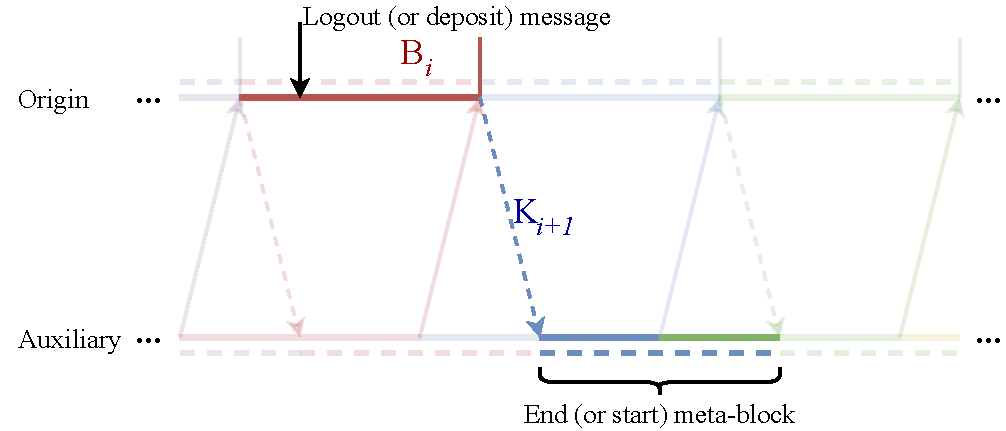
\includegraphics[width=0.8\textwidth]{dynamic_validators}
	\caption{\textbf{Dynamic set of validators.}
		The validator sends a log out (or deposit) message in $B_i$.
		The change in the set of validators is transferred to auxiliary as part of kernel $K_{i+1}$ when it gets confirmed.
		The validator does its last (first) round in the rear (forward) validator set of $\mathcal{V}_{\mathcal{B}_{i+1}}$ ($\mathcal{V}_{\mathcal{B}_{r,i+1}}$ or $\mathcal{V}_{\mathcal{B}_{f,i+1}}$ respectively).}
	\label{fig:dynamic_validators}
\end{figure}

\subsection{Beyond an honest supermajority}

While the origin blockchain protects assets from being double-spent, users in a meta-blockchain could see their funds stolen if more than a supermajority of the open validator set would collude to violate the transition rules $t_A$. 

We identify at least three active research topics which can allow to push the security model radically further in an efficient way; namely that (up to) a \emph{single} honest observer can hold all validators accountable when a proposal for committing a meta-block to the origin blockchain would violate the state transition rules $t_A$.
It is outside the scope of the current work to explore in-depth, but they are worth summarising below as future work paths.

\paragraph{observer network} In \textit{A Guide to 99\% Fault Tolerant Consensus}\cite{honestobserver} V. Buterin recaptures an existing algorithm by L. Lamport (1982) to describe how a \emph{latency-dependent} network of observers can be retrofitted on top of a \emph{threshold-dependent} consensus algorithm - in casu our here work as derived from Casper FFG - to introduce a \emph{strong-finality} upon the finalized history constructed by the Mosaic validators arbitrarily pushing up the fault-tolerance at the cost of requiring more observers and a longer time to eventually commit (a strongly finalized proposal).

\paragraph{truebit} A second worthwhile path is to apply the \textit{TrueBit}\cite{truebit} protocol to challenge a state transition $T^A$ proposed by a subset of the validators $\mathcal{V}_{\mathcal{B}_i}$.
The validators $\{v\}$ who have signed vote messages $\langle\tilde{T}^A, s, t, h_s, h_t\rangle_v$ can be seen as the (collective) \emph{solvers} of the off-(of-origin-)chain computation to transition the state $B_{n-1}$ to the proposed solution $s$ given the set of transactions specified by the accumulated transaction root $r_{h_s}$.
The computation at hand is the execution of the virtual machine that implements the state transition rules $t_A$.

If less than $\sfrac{1}{3}$ of the validator weight loses the verification game to a challenger, their stake can be taken as the reward for the challenger, on top of the shared interest of all participants in the meta-blockchain for only correct proposals to be committed to the origin chain - removing the need for a jackpot and a \emph{forced-error}.
The verification game can be seen as an extension to the slashing conditions strengthening the accountable safety of the meta-blockchain to hold a minority of the validators accountable for violating the state transition rules $t_A$.
This is made possible because the validator stake has been externalized on the origin blockchain with an independent (assumed correct) consensus mechanism.

If more than $\sfrac{2}{3}$ of the validator weight signed the vote message which was challenged and lost the verification game, their stake is the reward for the challenger, and the meta-blockchain must be declared halted by the core contract.

\paragraph{argument of knowledge} A third strategy can be constructed by requiring any of the challenged validators of a proposal $T^A$ to present an \emph{argument of knowledge}, eg. using \mbox{zkSNARKs} generated after being challenged, to cryptographically prove that the block $s$ has been obtained by correctly applying the state transition rules $t_A$ recursively on each parent block building up from the committed block found in $B_{n-1}$.

The costs both in time and expense to generate this proof by a validator scale at first approximation linearly with the gas consumed in the proposed meta-block $B_n$.
The transition object $T^A$ to commit this meta-block tracks the gas consumed, so the core contract can require that the challenger puts forward a sufficient stake to substantiate her claim.

% TODO: research state of art on hardware requirements
There are open considerations regarding the (economic) feasibility of requiring all validators to be able to generate such a proof on commodity hardware.
The task of generating these proofs could be designated to a specialized node, but an incentive problem arises when it is economically unattractive to run such a node considering it is unlikely that a proposal would be challenged.

We have gone beyond the assumption of an honest supermajority of validators by considering three strategies discussed in the field to radically improve the security model; up to the point where a single honest observer can cost-effectively challenge the validator set on the origin blockchain.

%
% Section
%
\section*{Conclusion}
We have constructed Byzantine fault-tolerant consensus rules for an open, dynamic validator set to compose transactions executed on an auxiliary system asynchronously into an origin blockchain, e.g. Ethereum mainnet.
Each commit on the origin blockchain by a supermajority of the validators can span an arbitrarily large measure of computation finalised on the auxiliary system. A working draft formulation of implementation work done on the gateway protocol is appended to this document.

\bibliographystyle{naturemag}
\bibliography{mosaic.bib}

\newpage

\begin{versionhistory}
  \vhEntry{0.0}{10.10.18}{*}{Asynchronous composition of blockchains (section 1 - 2.7)}
\end{versionhistory}

\newpage
\begin{center}
\rule{\textwidth}{.4pt}\par
{\huge\bfseries Working Draft \par}
\rule{\textwidth}{.4pt}\par
\bigbreak
{\Large ---proceed carefully---\par}
\end{center}


\subsection{gas markets}

A meta-blockchain has a double gas market.
First the known gas market exists where users of the auxiliary system pay gas fees to the block proposers of the auxiliary system for every transaction.
A second, new gas market is created that rewards validators for their work.

Validators must verify transactions of the origin blockchain and the auxiliary system.  They must cast vote messages to finalise checkpoints of the auxiliary system and observations of the origin blockchain on the auxiliary system.
Validators propose transition objects to the origin blockchain and commit meta-blocks based on these proposals.

Validators earn reward for their contribution to the construction of a finalised history on the auxiliary system.  A meta-block must be committed for the rewards earned on the auxiliary system to be realised on the origin blockchain.

We call $\{\sigma_i\}$ with $i \in [k_{1,n}, k_{N,n}]$ a \emph{segment} with $N$ supermajority links in a justified chain (in meta-block height $n$), when $\sigma_i = \langle T_i, s_i, t_i, h_{s_i}, h_{t_i} \rangle$ each have a supermajority $\mathcal{S}(\mathcal{V}_{\mathcal{B}_n})$ (eq. \ref{eq:supermajority}) and $\sigma_{i+1}$ connects\footnote{
  Define $\sigma'$ connects to $\sigma$ if $t = s'$ and $h_{t} = h_{s'}$.}
to $\sigma_i$ for $i \in [k_{1,n}, k_{N-1,n}]$.

The reward a validator $v$ earns over a segment $\{\sigma_i\}$ is
\begin{align}
    \frac{W_v}{w}\sum_{i} \Delta g_{i} \cdot gp_{d(i)} \cdot \delta_{1, v(i)}
\end{align}
where $W_v$ is the effective weight of the validator, $w = \sum_v w_v$ is the total weight of all validators, $\Delta g_{i}$ is the gas consumed from source to target, $gp_{d(i)}$ is the gas price agreed upon by block proposers for dynasty $d(i)$, and $\delta_{1, v(i)}$ is one when the validator $v$ had voted for $\sigma_i$\footnote{The validator vote must have been included when the rewards are calculated and awarded to the validators on the auxiliary system. We propose to calculate and transfer rewards when the justified chain is finalised.}
or zero otherwise.

Gas fees will be awarded in the base token of the auxiliary chain.

A smart contract on auxiliary manages the validator rewards.
Maximally 49\% of the rewards are paid out directly to the validator addresses.
The remaining 51\% are locked in until after the withdrawal period ends after a validator logged out.
If the validator violates a slashing condition, the withheld 51\% will be slashed along with the validator's stake.
More than half of the rewards are kept so that the paid out rewards never outweigh the potential loss in case of a violated slashing condition.

In order for the auxiliary smart contract to be able to handle these rewards, the block proposers of auxiliary must collectively deposit sufficient value for multiple future meta-blocks in the reward contract on the auxiliary system and keep replenishing this pre-deposit from the gas fees they earn from users through transaction fees.

Block proposers have to be staked on the auxiliary system in order to be able to vote on changes to the gas price in a given dynasty.
Validators for their turn must for multiple meta-block heights in advance commit to a minimum gas price.

The gas price in a given dynasty voted on by the block proposers cannot be lower than the minimum gas price committed to by the validators.
Block proposers can attract more validators to the meta-blockchain by raising their gas price.

Users of the auxiliary system paid a gas fee to the block proposers when their transactions were included in an auxiliary block.
Block proposers pay for a given dynasty a gas price $gp_d$ to the validators to verify and finalize the history of transactions.
Both block proposers and validators can only access their rewards on the origin blockchain if the finalised history is also committed.

In addition the gas target requires the validators to expend the cost of committing the finalised history on the origin blockchain, because failing to do so would incur loss on their stake.

%\subsection{Attacks and Defenses}
%
%We defend against the two main attacks against proof of stake systems the same way Casper FFG\cite{casperffg} does:
%\begin{itemize}
%    \item We defend against \emph{long-range revision} by introducing a \emph{withdrawal delay} and a \emph{maximum source block age} for votes.
%    \item We defend against \emph{catastrophic crashes} by introducing an \emph{inactivity leak}.
%\end{itemize}
%However, there are a number of new attack vectors introduced by the concepts of a meta-blockchain and decoupled systems:
%\begin{itemize}
%    \item Delaying kernel confirmation.
%    \item Reporting invalid blocks to the auxiliary system.
%    \item Validators produce votes to commit on origin without actually voting on auxiliary.
%    \item Validators stop finalizing.
%\end{itemize}
%
%
%\paragraph{Kernel delay.}
%The set of validators could have an interest in delaying the confirmation of a new kernel, e.g. to prevent a new validator from joining the set of validators.
%However, the system is designed in a way that anyone, even the new validator that is not yet part of the set of validators, can do the Merkle proof to confirm a new kernel on auxiliary.
%All that is required for that is a finalized checkpoint of origin on auxiliary that includes the state root that includes the commit of the previous kernel.
%If the validators delay origin block finalization to prevent the kernel opening, they would lose stake as the result of the inactivity leak.
%
%\paragraph{Invalid block reports.}
%Block reporting to auxiliary is not limited to any set of specific addresses.
%An adversary could report origin blocks that do not actually exist on origin.
%There is no way for auxiliary to check the validity of these reports.
%However, validators would ignore these reports and not vote on them, the adversary is only burning gas fees.
%
%\paragraph{Belated vote production.}
%Say someone proposes a transition object to origin for which a supermajority vote by the validators does not exist.
%Validators may produce votes to commit that proposal.
%There are two cases then to consider:
%
%\begin{enumerate}
%    \item The produced votes never violate any slashing condition.
%    \item The produced votes violate a slashing condition eventually.
%\end{enumerate}
%
%In the first case, the commit on origin is in-line with what is actually observed on auxiliary.
%In the second case, at least $\sfrac{1}{3}$ of the validators' stake can be slashed.
%
%\paragraph{Finalization breakdown.}
%If validators decided to stop finalization, they would lose stake due to the inactivity leak.
%

\newpage

%
% Section
%
\section{Gateway}\label{gateway}

Gateway protocol allows decentralized applications to move tokens between two heterogeneous blockchain systems. 
This protocol can be used to move token(ERC20, later non-fungible tokens) between origin blockchain and auxiliary system supporting a specific meta-blockchain where transactions can be finalized faster, and at a lower transaction cost. 
Gateway protocol leverages the idea of message bus which defines a standard to asynchronously transfer typed messages between two chains.
 
We define message bus $M_b$ as a state machine with messages $m_s$ where $s$ denotes state, outbox $o_b$ and inbox $i_b$ for each blockchain. Messages from source chain are kept in the outbox
 and once verified on target chain using Merkle proof, they are saved in the inbox of target chain. 
 
\begin{align}
  M_b  = (\{ m^1_s,m^2_s ... ,m^n_s \}, o_b, i_b)
\end{align}


Gateway contract is deployed on origin chain and twin contract co-gateway is deployed on an auxiliary chain. 
These two contracts are linked before initiating any message passing. 
Linking ensures that both contracts are set up to transfer the same token and use the same version of the message bus. 
Gateway and Co-gateway contracts defines different message types i.e. linking, stake \& mint and redeem \& unstake. 
Any facilitator can transfer messages between source and target blockchain by staking bounty as a security amount. 
Facilitator is rewarded by message initiator along with the bounty on successful completion of message transfers. 
\subsection{Message Bus}\label{gateway:messagebus}
    
The Message Bus is a messaging framework that allows to atomically communicate typed messages between two heterogeneous blockchain systems. 
This communication is a two-phase commit on each blockchain to move a message between blockchains. 
Message bus acts as a state machine where message state is changed from one state to another in response to interaction with message bus. 
If message $M$ is intended to move from blockchain $A$ to blockchain $B$, then in this case the $A$ is termed as the source and $B$ is termed as target.
The state of message $M$ is stored in outbox of source blockchain and in the inbox of target blockchain.
\begin{figure}[htb]
    \centering
	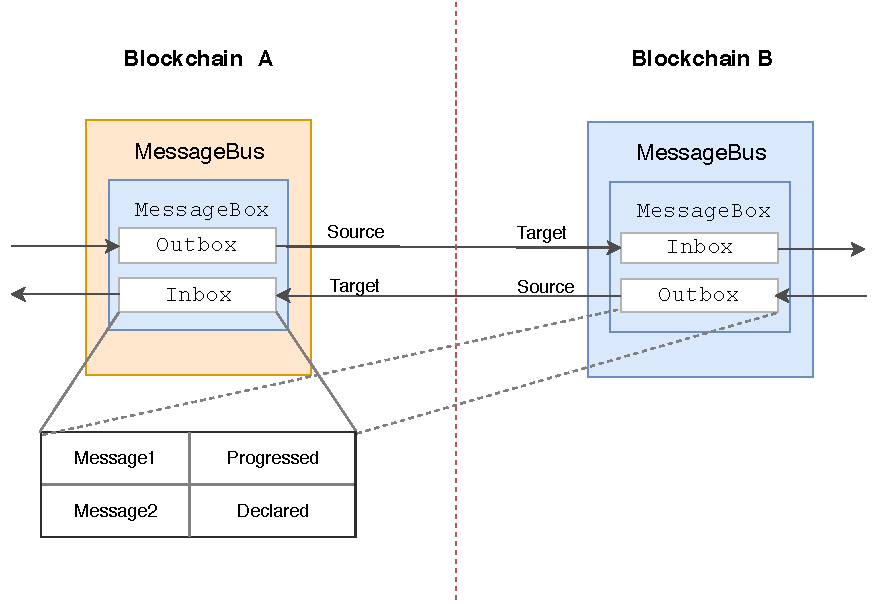
\includegraphics[width=\textwidth]{messagebus}
	\caption{\textbf{MessageBox of the MessageBus}}
	\label{fig:messagebus}
\end{figure}

Similarly if the message is intended to move from blockchain $B$ to blockchain $A$, then the source will be $B$ and target will be $A$.
Throughout the paper the terms source and target blockchain will be used.

\subsubsection{Message}\label{gateway:message}
We introduce message $M$ consists of message type intent hash $i_t$ where $t$ defines type of message, nonce $n$, gas price $g_p$ , gas limit $g_l$ , sender $s$, hash lock $h_l$. 
Nonce $n$ is the count of message moved from source blockchain to target blockchain by the sender $s$. 
Gas price $g_p$ and gas limit $g_l$  is the price at which the reward is calculated for facilitation of message transfer, refer section \ref{gateway:reward}  
Hash lock $h_l$ is a hash that is set by the facilitator, refer section \ref{gateway:progresshashlock} 
\begin{align}
  M = (i, n, g_p, g_l, s, h_l) 
\end{align}

Message hash $m_h$ is an unique identifier of a message $M$. It can be calculated as the hash of message type hash $t$, intent hash $i$ , nonce $n$, gas price $g_p$ , gas limit $g_l$ ,sender $s$ and $K$ is $keccak256$ hashing function. 
     
     \begin{align}
     	\tilde{m}_h = K(t, i, n, g_p, g_l, s) 
     \end{align} 

\subsubsection{State machine}\label{gateway:statemachine} 
Message bus acts as a state machine, the transition of message state is deterministic. 
The possible states $q$ of the message can be Undeclared $q_u$ , Declared $q_d$, Progressed $q_p$, RevocationDeclared $q_{rd}$  and Revoked $q_r$. 
\begin{figure}[htb]
    \centering
	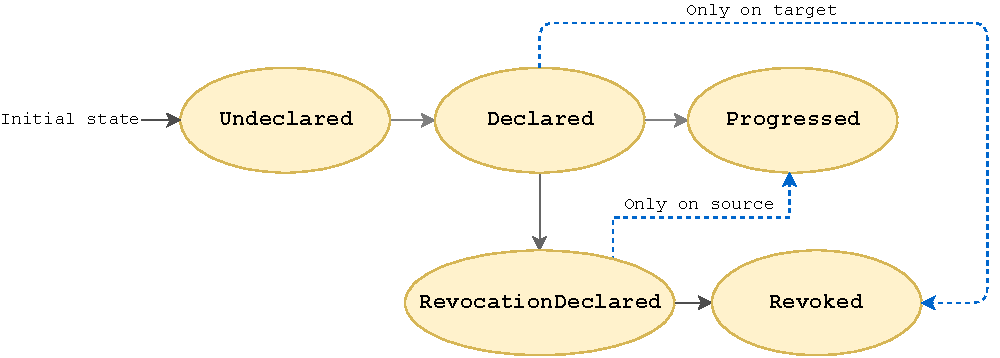
\includegraphics[width=\textwidth]{state_diagram}
	\caption{\textbf{States of the message}}
	\label{fig:state_diagram}
\end{figure}

Message $M$ can be moved from source blockchain to target blockchain in four steps consisting of two phased commit transactions in both blockchains each. 
This four steps are
\begin{enumerate}
\item Declare
\item Confirm
\item Progress outbox
\item Progress inbox
\end{enumerate}

\subsubsection{Declare}\label{gateway:declare}

We define state transition function \emph{declare message} $T_d$ on source blockchain which changes message state from undeclared $q_u$ to declared $q_d$, if signature $\langle \tilde{m}_h \rangle_s$ signed by message initiator $s$ is valid.

\begin{equation*}
T_d(M,\langle \tilde{m}_h \rangle_s)=\begin{cases}
q_u \rightarrow q_d & \text{if $\langle \tilde{m}_h \rangle_s$ is valid},\\
q_u& \text{otherwise}.
\end{cases}
\end{equation*}

Where $\langle \tilde{m}_h \rangle_s$ is signed message hash.

Declaration of message transfer happens in outbox of source blockchain on successful execution of state transition function declare.

\subsubsection{Confirm}\label{gateway:confirm}

We define state transition function \emph{confirm message} $T_c$ on target chain which changes message state from undeclared $q_u$ to declared $q_d$ if an valid merkle proof $p^s_{q_d}$ is presented stating message declaration on source chain.

\begin{equation*}
T_c(M,p^s_{q_d})=\begin{cases}
q_u \rightarrow q_d & \text{if $V$($p^s_{q_d}$) == true},\\
q_u& \text{otherwise}.
\end{cases}
\end{equation*}
\begin{align*}
\end{align*}
Where $p^s_{q_d}$ represents merkle proof $p$ for message status $q_d$ on source chain $s$ and $V$ is merkle proof verification function.

\subsubsection{Progress outbox}\label{gateway:progressoutbox}

We define state transition function \emph{progress outbox message} $T_p$ on source chain which changes message state from declared $q_d$ to progressed $q_p$, if an valid merkle proof $p^t_{q_d}$ is presented stating message declaration $q_d$ or message progressed $q_p$ on target chain $t$. 
Refer figure \ref{fig:progress_with_proof}. 

Once progressed state $q_p$ is achieved, message transfer can’t be revoked. 

\begin{equation*}
T_p(M,p^t_{q_d})=\begin{cases}
q_d \rightarrow q_p & \text{if $V$($p^t_{q_d}$) == true},\\
q_d& \text{otherwise}.
\end{cases}
\end{equation*}
\begin{align*}
\end{align*}

Where $p^s_{q_d}$ represents merkle proof $p$ for message status $q_d$ on source chain $s$ and $V$ is merkle proof verification function.

\subsubsection{Progress inbox}\label{gateway:progressinbox}

We define state transition function \emph{progress inbox message} on source chain which changes message state from declared $q_d$ to progressed $q_p$, if an valid merkle proof $p^s_{q}$ is presented stating message declaration $q_d$ or message progressed $q_p$ on source chain $s$.
 Once progressed state $q_p$ is achieved, message transfer can’t be revoked. Refer figure \ref{fig:progress_with_proof}. 

\begin{equation*}
T_p(M,p^s_{q})=\begin{cases}
q_d \rightarrow q_p & \text{if $V$($p^s_{q}$) == true},\\
q_d& \text{otherwise}.
\end{cases}
\end{equation*}
\begin{align*}
\end{align*}

Where $p^s_{q}$ represents merkle proof $p$ for message status $q_d$ or $q_p$ on source chain $s$  and $V$ is merkle proof verification function.

\begin{figure}[htb]
    \centering
	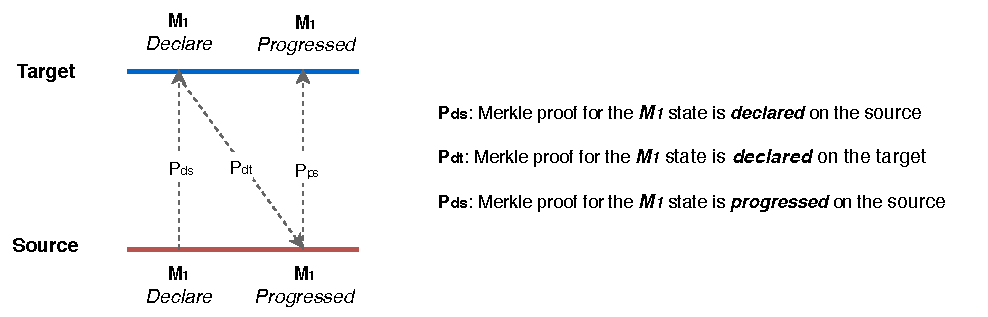
\includegraphics[width=\textwidth]{progress_with_proof}
	\caption{\textbf{Progress with proof}}
	\label{fig:progress_with_proof}
\end{figure}

\subsubsection{Progress with HashLock}\label{gateway:progresshashlock} 

Progress outbox  and progress inbox is a costly operation in terms of gas consumption as it involves merkle proof verification. 
So an alternative mechanism to complete progress outbox and progress inbox is \emph{progress with hash lock} $T_{phl}$  in both source and target blockchains. 
While declaring the message M, an hashlock $h_l$ can be provided in the message. We define hash lock $h_l$ as

\begin{align}
	h_l = K(s)
\end{align}

\begin{equation*}
T_{phl}(M,k_s)=\begin{cases}
q_d \rightarrow q_p & \text{if $K$($k_s$) == $\tilde{h}_l$},\\
q_d& \text{otherwise}.
\end{cases}
\end{equation*}
\begin{align*}
\text{where $K$ is hashing function $keccak256$}
\end{align*}

where $K$ is hashing function like $keccak256$, $k_s$ is a unlock secret 

Progress with hash lock can be used by presenting unlock secret on both chains. However, in some scenarios progress with hash lock can't be used. Refer section \ref{gateway:revocation}.

\begin{figure}[htb]
    \centering
	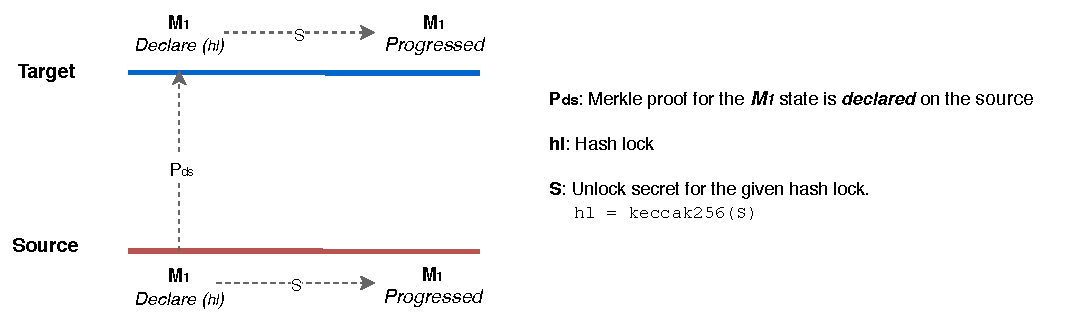
\includegraphics[width=\textwidth]{progress_with_hashlock}
	\caption{\textbf{Progress with hash lock}}
	\label{fig:progress_with_hashlock}
\end{figure}
\subsubsection{Revocation}\label{gateway:revocation}

We define state transition function \emph{revocation declaration} $T_{rd}$ on source blockchain which stops message transfer process. Revocation declaration $q_{rd}$ is done if message status is declared ${q_d}$.  
Only message initiator can declare revocation message $q_{rd}$  on source chain.

\begin{equation*}
T_{rd}(M)=\begin{cases}
q_d \rightarrow q_{rd} & \text{if revocation declaration is done by message initiator},\\
q_d& \text{otherwise}.
\end{cases}
\end{equation*}
\begin{align*}
\end{align*}

Message can directly be revoked on target chain without revocation declaration by presenting merkle proof specifying status revocation declaration $q_{rd}$ on source chain. If message is not declared ${q_d}$ on target chain before revocation then it should be first declared ${q_d}$.
 Refer figure \ref{fig:revocation}.

\begin{equation*}
T_{r}(M,p^s_{q_{rd}})=\begin{cases}
q_d \rightarrow q_{r} & \text{if $V$($p^s_{q_{rd}}$) == true},\\
q_d& \text{otherwise}.
\end{cases}
\end{equation*}
\begin{align*}
\end{align*}
Where $p^s_{q_{rd}}$ represents merkle proof $p$ for message status $q_{rd}$ on source chain $t$, $V$ is merkle proof verification function and $K$ is hashing function $keccak256$.

With \emph{revoked} $T_r$ state transition function,  message revocation can completed on source blockchain. Revoked status $q_r$ on source blockchain is only achieved, if state of message M on target blockchain is revoked $q_r$.

\begin{equation*}
T_{r}(M,p^t_{q_r})=\begin{cases}
q_{rd} \rightarrow q_r & \text{if $V$($p^t_{q_r}$) == true},\\
q_d& \text{otherwise}.
\end{cases}
\end{equation*}
\begin{align*}
\end{align*}

Where $p^t_{q_r}$ represents merkle proof $p$ for message status $q_r$ on target chain $t$, $V$ is merkle proof verification function and $K$ is hashing function $keccak256$.

 
On the source blockchain if the state of message is revocation declared $q_{rd}$ where as the status of message in target blockchain is progressed ${q_p}$, in this case the status on source blockchain can be changed only to progressed ${q_p}$ by state transition function \emph{progress outbox} explained in section \ref{gateway:progressoutbox}.

\begin{figure}[htb]
    \centering
	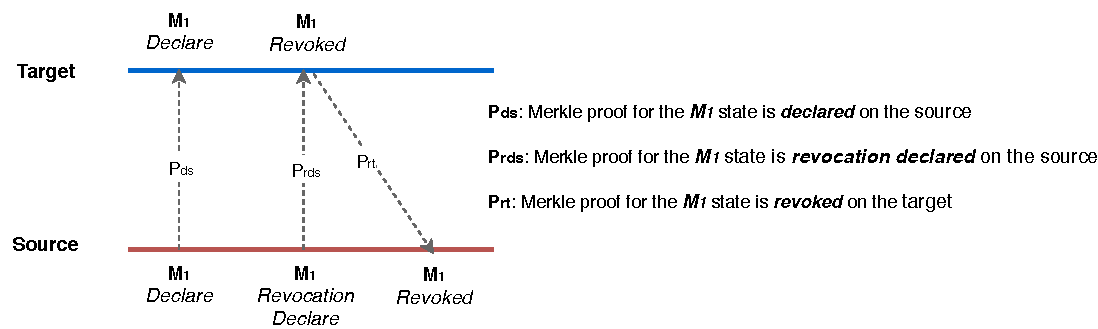
\includegraphics[width=\textwidth]{revocation}
	\caption{\textbf{ Revocation of message}}
	\label{fig:revocation}
\end{figure}


\begin{figure}[htb]
    \centering
	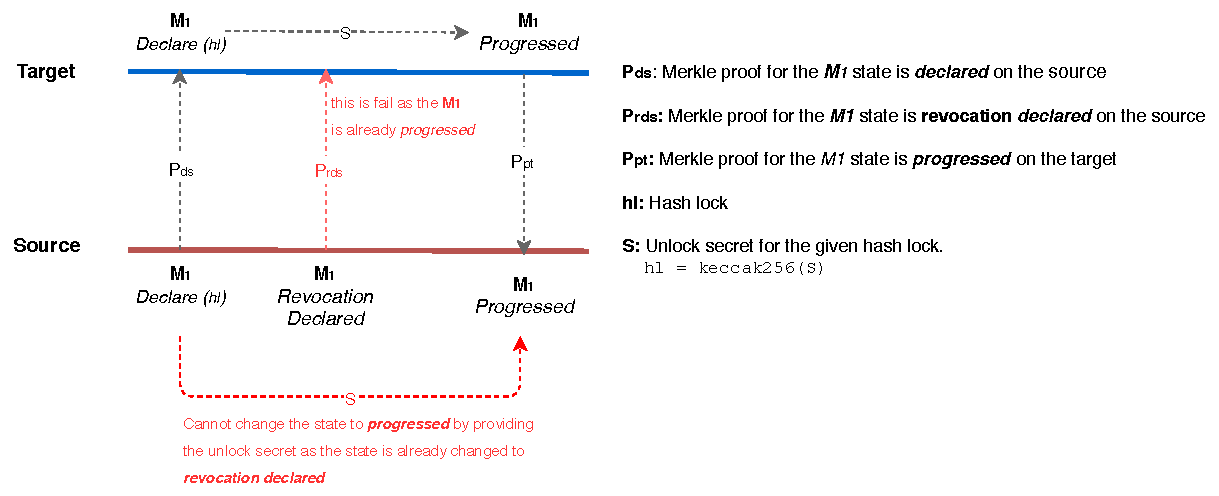
\includegraphics[width=\textwidth]{revocation_progress}
	\caption{\textbf{ Progress after revocation declared.}}
	\label{fig:revocation}
\end{figure}

\subsection{Linking of Gateway and Co-Gateway}\label{gateway:linking}
Gateway is defined on origin blockchain where as Co-gateway defined on auxiliary blockchain and can co-exists only in pair to be functional. 
Both the contracts are inactive by default i.e both the contracts cannot transfer any messages except linking messages.
 
 Linking of Gateway and Co-gateway is a special type of message transfer which cryptographically verify uniformity of token and message bus on origin and auxiliary blockchain. 
 As explained in section \ref{gateway:messagebus}, each message contains message type intent hash. 
 For linking messages, we define gateway linking intent hash $i_{gl}$ as a hash of gateway address $g_a$, co-gateway address $c_a$, message bus code hash $m_{ch}$, ERC20 token name $t_n$, token symbol $t_s$, token decimal $t_d$, nonce $n$, token address $t_a$ and $K$ is $keccak256$ hashing function.
 \begin{align}
i_{gl}  =K(g_a, c_a, m_{ch}, t_n, t_s, t_d, n, t_a) 	
 \end{align}

Once the linking message is declared in gateway, it can be confirmed on co-gateway by merkle proof. 
After completion of the progress the Gateway and Co-gateway are activated and can perform the other message transfers like stake \& mint or redeem \& unstake. 

\subsection{Stake and Mint}\label{gateway:stakemint}
Gateway protocol supports transfer of stake and mint type typed message from origin to auxiliary chain. 
Staking happens on origin chain which locks staker’s tokens into the escrow and miniting happens on auxiliary chain which creates new tokens at beneficiary address. 
By combining meta-blockchain based layer 2 scaling solution with this message type, a token economy can be designed with the high transaction throughput and low gas cost on auxiliary chain.

Staker needs to submit a signed message hash to facilitator to initiate message transfers. 
As described in section \ref{gateway:message}, message hash generation needs message type specific intent hash which is staking intent hash $i_s$ in this scenario . We define staking intent $i_s$  as : 
 \begin{align}
 	s = K(a_s,b_a,s_a,n_s,g_p,g_l,t_a )
 \end{align}
                                                       
Where $K$ is $keccak256$ hashing function, $a_s$ is staking amount, $b_a$ is beneficiary address, $s_a$ is staker address, $n_s$ is staker nonce, $g_p$ and $g_l$ are gas price and gas limit respectively as described in section \ref{gateway:reward}, $t_a$ is ERC20 staking token address. 

Gateway along with message bus verifies staker’s signature generated by signing message hash and initiates message transfer.
Facilitator must stake bounty to gateway during message declaration on source chain as described in section \ref{gateway:bounty} 

Message declared on origin chain with staking intent hash is verified and confirmed on auxiliary chain with merkle proof. 
Tokens are minted for beneficiary on auxiliary blockchain after successful progress. 
On successful mint of token, reward is awarded to facilitator from the minted token refer section \ref{gateway:reward}.

\subsection{Redeem \& Unstake}\label{gateway:redeemunstake}

Gateway protocol allows unstake of the tokens by moving the tokens back from auxiliary chain to origin chain. 
The tokens from redeemer address $s_a$ in auxiliary chain is moved to beneficiary address $b_a$ in the origin chain. 
This is done with the transfer of redeem \& unstake typed message $M$ through the message bus.

To create a message $M$, we use the redemption intent hash $\tilde{i}_r$ as:
 \begin{align}
 \tilde{i}_r = K(a_r,b_a,s_a,n_s,g_p,g_l,t_a )    
 \end{align}

Where $K$ is \emph{keccak256} hashing function, $a_r$ is staking amount, $b_a$ is beneficiary address, $s_a$ is redeemer address, $n_s$ is redeemer nonce, $g_p$ and $g_l$ are gas price and gas limit respectively as described in section \ref{gateway:reward}, $t_a$ is ERC20 staking token address. 

On Message $M$ declaration on the auxiliary chain, $a_r$ amount of redeemer's token is moved to escrow in auxiliary chain. Message $M$ is verified and confirmed on origin chain with merkle proof.

On successful progress of message in the auxiliary chain, the $a_r$ amount of tokens from the escrow are burnt.Whereas on the successful progress of message in the origin chain, the $a_r$ amount of tokens are transferred from the staked pool of tokens to the beneficiary address.

\subsection{Bounty}\label{gateway:bounty}
 In Gateway protocol, facilitator pool is an open network of nodes which are responsible for message transfer between source and target chain. 
 Any node/machine can act as facilitator by staking bounty to gateway during message transfer. 

Bounty is the fixed amount staked by facilitator as a security deposit during message transfer.
This amount should be just sufficient to maintain the accountability for message transfers by facilitator. 
Facilitator must approve gateway for bounty amount before declaring message. 
Bounty enforces facilitator to progress on source chain. 
It is returned back to facilitator who reveals unlock secret or progresses with the proof.

If message initiator(staker or redeemer) decides to revoke message transfer, it has to pay penalty described in section \ref{gateway:penalty}. 
Both bounty and penalty are burned on progress revocation. 

\subsection{Reward}\label{gateway:reward}
Gateway protocol has reward structure for facilitator for successful completion of message transfers. 
Section \ref{gateway:messagebus} explains the four step process to transfer message from source to target blockchain. 
Facilitator presents hash lock during message declaration on source blockchain. 
When the correct unlock secret is presented on target blockchain during progress, facilitator is rewarded with reward $r$. 

We define reward $r$ as following:
 \begin{align}
 	r  = g_p  *  min(g_l, g_c + K) 
 \end{align}
                         
Where $g_p$ is gas price, $g_l$  is gas limit,  $K$ is constant and $g_c$  is measured gas consumption over merkle proof verification. $g_c$ is the sum of gas spent in declaring inbox message $g_d$ and progressing inbox $g_p$ and can be defined as :
 \begin{align}
 	g_c  = g_d  + g_p
 \end{align}
                                     
$g_p$ and $g_l$ is decided by message initiator which determines maximum reward amount $r_{max}$
 \begin{align}
 	r_{max}  = g_p *  g_l
 \end{align}

\subsection{Penalty}\label{gateway:penalty}
Penalty is the amount charged to message initiator for revocation of message transfer. 
Penalty is charged when initiator decides to revoke message after declaration and before progress.  
In order to ensure a fair and honest process between the facilitator and the initiator, the penalty charge must always be greater than the bounty amount.  

Penalty P for message transfer revocation is:
 \begin{align}
 	P = n * b_f
 \end{align}
                                           
Where $n > 1$  and $b_f$ is bounty staked by facilitator. 

\subsection{Gateway deactivating}\label{gateway:deactivating}
The transfers of message from Gateway to Co-gateway can be restricted by deactivating the Gateway.
No new message can be transferred where as existing message can still be transferred.
This does not restricts the message transfer from Co-gateway to Gateway. 
The tokens can be still redeemed with gateway deactivating.

\subsection{Chain halting}
                                                            
%
% Section
%
\section{A mosaic of cores}

summary:
By constructing asynchronous BFT consensus rules to compose a heterogeneous auxiliary blockchain into the origin blockchain, we leverage the security of the origin blockchain to asynchronously finalize the transactions on the auxiliary blockchain.
As there are no time constraints or time-outs in the Mosaic consensus rules, the limited processing capacity of the origin blockchain does not undercut the ability to compose many auxiliary systems into the same origin blockchain.
This enables Mosaic to run many meta-blockchains in parallel, additively improving the total transaction capacity, but keeping a bound on the cost imposed on the origin blockchain.

\subsection{On data withholding attacks}
%
% Section
%
%\section{Outlook}

%
% Section
%
%\section{Conclusion}

%\section{Appendix}





\end{document}
